\section{ACL en use}

Dans cette session on verrais les uses des ACL dans les système d'aujourd'hui. 

\subsection{ACL Kernel Patches}
Les ACL \emph{patches} ont été ajouter dans le noyaux Linux depuis November 2002. Cette \emph{patches} implémentent le POSIX 1003.1e brouillon 17 et elles ont été ajoute dans le version 2.5.46 du noyaux. Donc le support ACL et aussi présent dans le dernière version du noyaux aujourd'hui. Depuis 2004 le support aux ACL étions disponible pour les système de fichier Ext2, Ext3, IBM JFS, ReiserFS et SGI XFS. Les ACL sont supporte aussi pour le système NFS, par contre, il y a quelques problèmes de sécurité connu\cite{nfs_problem}. 

Aujourd'hui c'est assez simple pour ajouter le supporte aux ACL dans les distribution Linux comme Ubuntu ou Debian. On verrais les pas pour ajouter ce supporte après.

\subsection{Mac OSX}
Le système de exploitation Mac OSX (10.6.2 Snow Leopard dans le moment de écriture de ce article) a aussi les supporte aux ACL complètement intégrée dans l'interface de utilisateur (\ref{fig:img_mac-acl}). 

\begin{figure}[htbp]
	\centering
		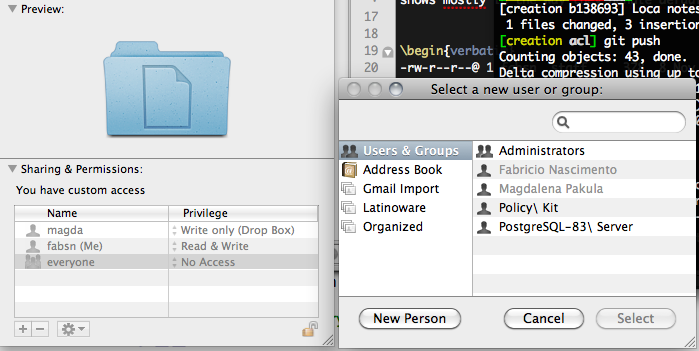
\includegraphics[height=3in]{img/mac-acl.png}
	\caption{Mac OSX Snow Leopard ACL Interface}
	\label{fig:img_mac-acl}
\end{figure}


%Parler un peut plus de Mac.


\subsection*{Using ACL in Linux}


%References 
Les dernière version des distribution Debian ou Ubuntu, comme Ubuntu 9.10, dèjá vient avec le supporte aux ACL. Dans le Ubuntu 8.10 l'application Nautilus, qui est responsable pour la visualisation du système de fichier, contenait une interface pour les ACL, apparentement l'interface a été discontinue et le Nautilus du Ubuntu 9.10 n'en y a pas encore. Les pas pour ajouter le supporte dans le Ubuntu 9.10 sont:

\begin{verbatim}
1) Installer le paquet des acl. 
user@ubuntu:$ sudo apt-get install acl
 
2) Ajouter le option 'acl' au système de fichier correcte dans le /etc/fstab, comment:
UUID='gros sequence' /dev/hda6 /home ext3 rw,auto,acl 0 1

3) Remounter le systeme de fichier avec le nouvelle option
user@ubuntu:$ sudo mount /home -o remount

\end{verbatim}

\subsection*{Ajouter ACL aux fichiers}

On peut utiliser le commande 'ls -la' pour regarde les permission. Si une fichier contient information de sécurité avancée (comme \emph{access list}) on va voir le "character" '+', comment dans le sortie du command 'ls' ci-dessous (\ref{verb:ls}). Une fichier avec '@' était dire que le fichier a quelque EAs. 

\begin{center}
\label{verb:ls}
\begin{verbatim}
-rw-r--r--@ 1 fabsn  staff     378  8 Nov 15:29 Makefile
-rw-r--r--@ 1 fabsn  staff     618  8 Nov 15:59 README
-rw-r--r--@ 1 fabsn  staff      31  8 Nov 15:15 draft-header
-rw-r--r--@ 1 fabsn  staff      24  8 Nov 15:15 header
drwxr-xr-x@ 2 fabsn  staff     102  8 Nov 15:26 img
-rw-r--r--  1 fabsn  staff     972  8 Nov 15:57 rapport-draft.aux
-rw-r--r--  1 fabsn  staff   18129  8 Nov 15:57 rapport-draft.log
drwxrwxr-x+ 3 fabsn  staff	  1024  8 Nov 20:23 repertoire
\end{verbatim}
\end{center}

Pour voir les ACL on doit utilise le commande \emph{getfacl}. Regarde que les information sont ajoute d'accord avec les définition dans l'introduction sur les ACL dans la tabelle \ref{tab:entree}. 

\begin{verbatim}
fabsn@vadmin:/media/esisar$ getfacl repertoire/
# file: repertoire/
# owner: root
# group: root
user::r-x
user:daemon:rwx
user:bin:rwx
user:fabsn:rwx
user:nobody:rwx
group::r-x
group:admin:rwx
group:fabsn:rwx
mask::rwx
other::r-x	
\end{verbatim}

Aussi on a le commande \emph{setfacl} pour modifier, ou ajouter les permission ACL. Le commande dessous par exemple modifie (-m) les permission du utilisateur \emph{fabsn} pour le répertoire. 

\begin{verbatim}
setfacl -m u:fabsn:r-x repertoire
\end{verbatim}

\subsection*{Exemple}

Voici une exemple d'utilisation trouvable dans le article d'Andreas Gruembacher\cite{aclsuse}.

On parte de la création de un répertoire avec l'application de umask de valeur 027 (octal). Ça veut dire que il va   désactiver l'écriture pour le groupe propriété et l'écriture, la lecture e l'exécution pour les autres.

\begin{verbatim}
$ umask 027 
$ mkdir dir 
$ ls -dl repertoire
	drwxr-x--- ... user group ... repertoire
\end{verbatim}

La lettre "d" montre que on l'objet "répertoire" c'est une répertoire suivi pour les octet de permission "rwxr-x---". Les réticences dans le command supprime les information avec aucune pertinence pour cette exemple. Cette permission basic on toujours une représentation dans les ACL, pour les afficher on faire:

\begin{verbatim}
$ getfacl repertoire
# file: repertoire 
# owner: user 
# group: goup
user::rwx
group::r-x
other::---
\end{verbatim}

Le trois première ligne après le commande (démarrer pour le \#) nous donne les information sur les propriétaire (groupe e utilisateur) et le nom du fichier. Après chaque ligne vient la liste des ACL. Ce exemple montre une ACL minimale. Si par exemple on ajoute permissions pour le utilisateur "jean" avec le commande \emph{setfacl} on va avoir les ACL étendu.

\begin{verbatim}
$ setfacl -m user:jean:rwx repertoire
$ getfacl --omit-header repertoire 
	user::rwx 
	user:jean:rwx	
	group::r-x 
	mask::rwx 
	other::---
\end{verbatim}

Il faut rappeler que le command \emph{setfacl} a été employer avec le modificateur \emph{-m (modify)}. Pour regarder les résultat on utilisé une autre fois le \emph{getfacl}. Il faut savoir que le modificateur \emph{--omit-header} cache les première 3 ligne avec les information sur les propriétaires.  

Tout d'abord on peut voir que l'entrée masque a été ajouter avec l'entrée d'utilisateur jean. Ces permission sont crée comme la union entré les permission de jean et du groupe propriétaire. La masque doit être une valeur que ne masque aucune permission, alors, ce valeur se trouve comme l'union de les élément que définissions la classe groupe.  

\begin{verbatim}
ls -dl repertoire
	drwxrwx---+ ... user group ... repertoire
\end{verbatim}

Si on rappel le dernière exemple, le groupe propriétaire n'y a pas le droit de écriture (\emph{group::r-x}), par contre, les groupe classe vient avec ce droit. C'est pour ça que quand on calcule effectivement le droit pour le groupe propriétaire dans le modèle acl, ce droit est toujours le union avec la masque.

Le prochaine exemple montre comme lest ACL sont modifiée pour l'emploie du command \emph{chmod} ou \emph{setfacl}. On va effacer le permission de écrit de la classe groupe. On doit voir que si il n'y a pas de masque, le command doit changer directement les permission dé l'entrée ACL du groupe propriétaire. 


\begin{verbatim}
$ chmod g-w repertoire 
$ ls -dl repertoire 
	drwxr-x---+ ... user group ... repertoire 
$ getfacl --omit-header repertoire 
user::rwx 
user:jean:rwx 	#effective:r-x
group::r-x 	
mask::r-x 
other::---

\end{verbatim}

Si une ACL entrée contient permission désactivé pour le masque, getfacl doit ajouter une commentaire qui montre ça différence. Il faut voir aussi qu'est-ce que se passe quand on rajoute le permission. 

\begin{verbatim}
$ chmod g+w repertoire 
$ ls -dl dir drwxrwx---+ ... user group ... repertoire 
$ getfacl --omit-header repertoir 
user::rwx 
user:jean:rwx 
group::r-x
mask::rwx
other::---
\end{verbatim}

After adding the write permission to the group class, the ACL defines the same permissions as before taking the permission away. The chmod command has a nonde- structive effect on the access permissions. This preserva- tion of permissions is an important feature of POSIX.1e ACLs.




%Default acl

\begin{verbatim}
$ setfacl -d -m group:group:r-x dir 
$ getfacl --omit-header repertoire 
user::rwx
user:jean:rwx
group::r-x 
mask::rwx
other::---
default:user::rwx
default:group::r-x
default:group:toolies:r-x
default:mask::r-x
default:other::---
\end{verbatim} 
% Following the access ACL, the default ACL is printed with each entry prefixed with “default:”. This out- put format is an extension to POSIX.1e that is found on Solaris and Linux. A strict implementation of POSIX 1003.2c would only show the access ACL. The default ACL would be shown with the -d option to getfacl.
% We have only specified an ACL entry for the toolies group in the setfacl command. The other entries required for a complete ACL have automatically been copied from the access ACL to the default ACL. This is a Linux- specific extension; on other systems all entries may need to be specified explicitly.
% The default ACL contains no entry for Joe, so Joe will not have access (except possibly through group member- ship or the other class permissions).
% A subdirectory inherits ACLs as shown next. Unless otherwise specified, the mkdir command uses a value of 0777 as the mode parameter to the mkdir system call, which it uses for creating the new directory. Observe that both the access and the default ACL contain the same entries.
% $ mkdir dir/subdir $ getfacl --omit-header dir/subdir user::rwx group::r-x group:toolies:r-x mask::r-x other::--- default:user::rwx default:group::r-x default:group:toolies:r-x default:mask::r-x default:other::---
% Files created inside dir inherit their permissions as shown next. The touch command passes a mode value of 0666 to the kernel for creating the file.
% All permissions not included in the mode parameter are removed from the corresponding ACL entries. The same has happened in the previous example, but there was no noticeable effect because the value 0777 used for the mode parameter represents a full set of permissions.
% Submitted for publication at the USENIX Annual Technical
% Conference, San Antonio, Texas, June 2003	5
% #effective:r-x
% $ touch dir/file $ ls -l dir/file -rw-r-----+ ... agruen suse ... dir/file $ getfacl --omit-header dir/file user::rw- group::r-x group:toolies:r-x mask::r-- other::---
% No permissions have been removed from ACL entries in the group class; instead they are merely masked and thus made ineffective. This ensures that traditional tools like compilers will interact well with ACLs. They can create files with restricted permissions and mark the files executable later. The mask mechanism will cause the right users and groups to end up with the expected per- missions.
% 





% # file: repertoire/
% # owner: root
% # group: root
% user::rwx
% user:daemon:rwx			#effective:r--
% user:bin:rwx			#effective:r--
% user:sys:rwx			#effective:r--
% user:sync:rwx			#effective:r--
% user:man:rwx			#effective:r--
% user:uucp:rwx			#effective:r--
% user:proxy:rwx			#effective:r--
% user:list:rwx			#effective:r--
% user:irc:rwx			#effective:r--
% user:gnats:rwx			#effective:r--
% user:syslog:rwx			#effective:r--
% user:klog:rwx			#effective:r--
% user:gdm:rwx			#effective:r--
% user:saned:rwx			#effective:r--
% user:pulse:rwx			#effective:r--
% user:avahi:rwx			#effective:r--
% user:sshd:rwx			#effective:r--
% user:fabsn:rwx			#effective:r--
% user:nobody:rwx			#effective:r--
% group::r-x			#effective:r--
% group:list:rwx			#effective:r--
% group:irc:rwx			#effective:r--
% group:src:rwx			#effective:r--
% group:shadow:rwx		#effective:r--
% group:utmp:rwx			#effective:r--
% group:video:rwx			#effective:r--
% group:lpadmin:rwx		#effective:r--
% group:crontab:rwx		#effective:r--
% group:pulse:rwx			#effective:r--
% group:avahi:rwx			#effective:r--
% group:haldaemon:rwx		#effective:r--
% group:admin:rwx			#effective:r--
% group:fabsn:rwx			#effective:r--
% mask::r--
